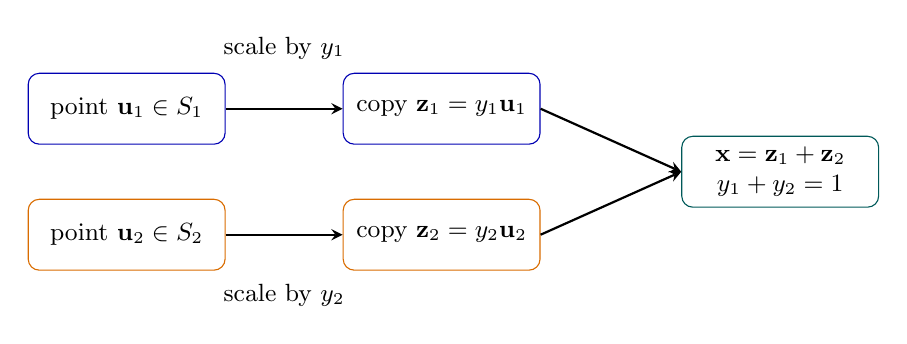
\begin{tikzpicture}[>=stealth,box/.style={draw,rounded corners,align=center,font=\small,minimum height=.9cm,minimum width=2.5cm}]
\node[box,draw=blue!70!black](a)at(0,.8){point $\mathbf u_1\in S_1$};
\node[box,draw=orange!85!black](b)at(0,-.8){point $\mathbf u_2\in S_2$};
\node[box,draw=blue!70!black](c)at(4,.8){copy $\mathbf z_1=y_1\mathbf u_1$};
\node[box,draw=orange!85!black](d)at(4,-.8){copy $\mathbf z_2=y_2\mathbf u_2$};
\node[box,draw=teal!70!black](x)at(8.3,0){$\mathbf x=\mathbf z_1+\mathbf z_2$\\$y_1+y_2=1$};
\draw[->,thick](a)--node[above=5mm,font=\small]{scale by $y_1$}(c);
\draw[->,thick](b)--node[below=5mm,font=\small]{scale by $y_2$}(d);
\draw[->,thick](c.east)--(x.west);\draw[->,thick](d.east)--(x.west);
\end{tikzpicture}
